\documentclass{Resources/netsci-project}


% :::~ This is the configuration for the bibliography. DO NOT CHANGE
\usepackage[
    backend=biber,
    style=authoryear,
    natbib=false,
    maxcitenames=2,
    minbibnames=1, maxbibnames=99, 
    url=false, 
    doi=true,
    ]{biblatex}
    
    
\addbibresource{bib.bib}

\subjectarea{Network Science}

\begin{document}
\firstpage{1}

\title{Temporal Bow-Tie Component Analysis of the Bitcoin Transaction Network}
\author{Huang Chuanshan (Matriculation Number), Kunam Lutharsanen (Matriculation Number), Leupp Joël (Matriculation Number), Mrugala Hubert (Matriculation Number)}
\course{Network Science}
\school{Faculty of Business, Economics and Informatics}
\date{16 December 2020}

\maketitle

\begin{abstract}
Bitcoin has dominated the cryptocurrency market since its theoretical dawn in 2008, giving rise to numerous intriguing studies in different fields. In this project, we present a novel perspective of understanding the dynamics of bitcoin transaction network by performing a bow tie analysis. The evolution of the bow tie, as well as the relationship between different compartments is demonstrated. Furthermore, we introduce a Markov Chain model to formulate the interaction of nodes. 

\end{abstract}

\section{Introduction}

Bitcoin is a cryptocurrency backed with public and private key encryption that makes every record of transaction public and verifiable \autocite{Nakamoto2008}. Users can make transactions to each other by using Bitcoin (BTC) as the currency. A bitcoin network is hence established, with users as nodes and transactions as weighted directed edges.  

Due to the bitcoin peer-to-peer, cryptographic architecture, the network's nodes store a complete list of past transactions. Easily accessible data recorded on public ledgers can then be used to analyze this digital currency. There is some relevant previous work that investigates the bitcoin network with reference to network science. Notably, \textcite{Lischke2016} and \textcite{Baumann2014} explore bitcoin transaction network with basic descriptive statistics and network science specific metrics. Moreover, \textcite{Kondor2014} look at microscopic link formation and temporal wealth distribution in the bitcoin network.

Throughout this project, we are interested in extracting meaningful information from the bitcoin network. To achieve this, we perform a temporal bow tie component analysis on our network. [WHAT ELSE DO WE EXACTLY DO / WHERE THE DATA COMES FROM / DATA TIME FRAME]

[WORDING TO BE POLISHED] In this report we will present several further inspection based on Bow-tie analysis. First we fetch the network at evenly chosen time slots and sort them into compartments according to the Bow-tie categorization algorithm. The distribution of nodes into different compartments. [...]

\section{Bow-tie structure of a network}

Real-world networks are very different form theoretical graphs or random models of networks. Many tools, like centralities and community detection algorithms, can be used to study the inner structure of these complex networks. However, for directed networks, there is one very interesting approach that can be used to depict and describe an overall structure of a complex network. Such an approach is analyzing a network by using a "bow tie" structure. First to use bow-tie structure were \textcite{Broder2000} who analyzed the graph structure of the World Wide Web.

Bow-tie structure consists of a 'giant strongly connected' component (GSCC), 'in' component (IN), 'out' component (OUT). There are also tubes, inner tendrils, outer tendrils and disconnected components. The main components: SCC, IN and OUT are unsurprisingly illustrated as a bow tie with SCC as the knot. Every component except disconnected components are collectively called a giant weakly connected component (GWCC). GSCC is the core of the network where every node is reachable from any other. In IN component there exist a path between any node in IN and GSCC, but IN nodes cannot be reached from GSCC. OUT component nodes are also connected with the core and are reachable from GSCC but not the other way around. Tubes represent nodes which are reachable from IN and 'go' directly to OUT, thus there exist a path between the two compartments but its nodes are not connected to GSCC. Inner tendrils and outer tendrils are nodes that are reachable form IN or OUT respectively, but are not connected to any other component. Finally, disconnected components' nodes are connected only within themselves and do not belong to GWCC. 

\begin{figure}[h!]
%    \centering
    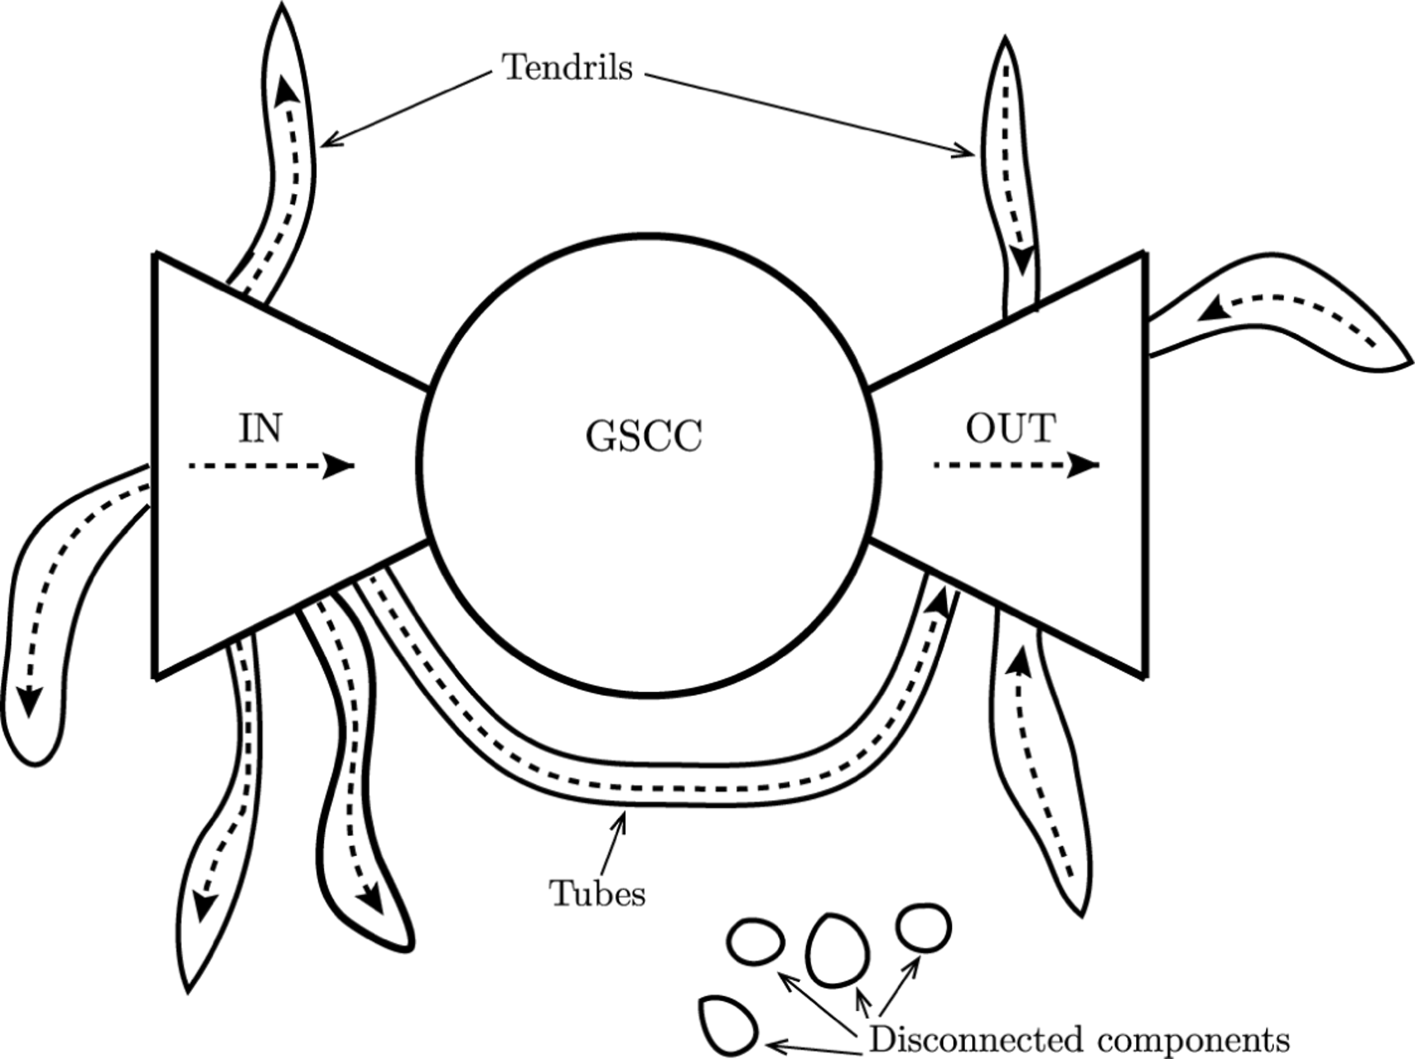
\includegraphics[width=\linewidth]{Resources/bowtie.png}
    \caption{A graph bow tie structure \autocite{Fujita2019}} 
    \label{fig:bowtie1}
\end{figure}

Since \textcite{Broder2000} the bow tie structure have been applied to explain macroscopic behavior of many complex networks ranging from social, e.g. online dating network \autocite{Chen2011}, to biological, e.g. bacterial metabolic architecture \autocite{Csete2004}. Bow tie can be also used to describe microscopic structures, where local bow ties can be found \autocite{Mattie2018, Fujita2019}. It is also worth to mention \textcite{Vitali2011} who use the bow tie to analyze control flows of transnational corporations, where the core is composed of a small highly connected clique of financial institutions.

As far as application of bow tie structure to blockchain systems, \textcite{Fujiwara2020} analyze 6-month transaction flows by using Helmholtz-Hodge-Kodaira decomposition and the bow-tie structure. \textcite{Guo2019} describe statistics of Ethereum transaction network, including bow tie components. \textcite{Maesa2019} evaluate macroscopic properties of bitcoin transaction network by studying the network's connectivity components and their temporal transformation in the bow tie framework. Our work also includes bow tie time analysis of the network components. However, our approach, on top of time series analysis as done in \textcite{Maesa2019}, includes a  Markov Chain model to investigate how bitcoin network actors change their location in the graph topology. Consequently, we can infer how economic actors' activity varies as the network evolves over time. 

\section{Method}

\section{Results}

\subsection{Basic statistics of the network}

\subsection{Time series component analysis}

\subsection{Markov Chain component transitions}

\section{Conclusion}

\printbibliography

\end{document}
